\documentclass[a4paper,italian,12pt,oneside]{book}
%%%%%%%%%%%%%%%%%%%%%%%%%%% Various package %%%%%%%%%%%%%%%%%%%%%%
% AMS mathematical packages

\usepackage{amsmath}
\usepackage{amsthm}
\usepackage{amsfonts}
\usepackage{longtable}
\usepackage[font=footnotesize, labelfont=bf]{caption}


% standard graphics package plus subfigure package
%\usepackage{psfig}
%\usepackage{epsf}
%\usepackage{epsfig}
\usepackage{graphicx}

% standard color graphics
\usepackage{color}
\usepackage{array}
\usepackage{colortbl}

% use Italian
\usepackage[italian]{babel}

% italian accentuated letters
\usepackage[applemac]{inputenc}

%Palatino like font
%\usepackage[T1]{fontenc}
%\usepackage{pxfonts}

%Latin Modern font
\usepackage{lmodern}
\usepackage[T1]{fontenc}
\usepackage{textcomp}

% headers customization
%\usepackage{fancyheadings}
%\usepackage{fancybox}
\usepackage{fancyhdr}
\pagestyle{fancy}

% the very first page!
\usepackage{frontpage}

%%%%%%%%%%%%%%%%%%%%%%%%%%%%%%%%%%%%%%%%%%%%%
\renewcommand{\topfraction}{.95}
\renewcommand{\textfraction}{.05}
\renewcommand{\floatpagefraction}{0.95}
%
\include{macros}

% interlinea
\linespread{1.5}

%PDF stuffs (hyperlinks)
%\usepackage[pdfauthor={Lorenzo Rotteglia},%
%            pdftitle={Elaborazione Di Mappe Acustiche Tramite Array Microfonici},%
%            pdftex]{hyperref}
%\hypersetup{colorlinks=false}

%%%%%%%%%%%%%%%%%%%%%%%%%%%%% Document Start %%%%%%%%%%%%%%%%%%%%%%%%%%%%%%%%
\begin{document}
%
\pagenumbering{roman}
\setcounter{page}{1}
%
\title{Elaborazione Di Mappe Acustiche\\[5mm] Tramite Array Microfonici\\}
\providecommand{\autore}{LORENZO ROTTEGLIA}                        %candidato
\providecommand{\principaladviser}{ANGELO FARINA}  %relatore
\providecommand{\firstreader}{SIMONE CAMPANINI}            %correlatore
\providecommand{\annoacc}{2012--2013}
\providecommand{\corso}{\uppercase{Informatica}} % corso di laurea in ??
\providecommand{\chiarmoprof}{Chiar.mo Prof.}
\providecommand{\dotting}{Dott. Ing.}
\providecommand{\dott}{Dott.}

\titlep

% PAGE HEADERS 
\pagestyle{fancy}
\renewcommand{\chaptermark}[1]{\markboth{{\chaptername}\ \thechapter.\hspace{1em}#1}{}}
\fancyhf{}
% definisce l'header e il footer
%\lhead[\fancyplain{}{}]{\fancyplain{}{\leftmark}} \chead{} \rhead{\thepage}
\fancyhead[RO,RE]{\nouppercase{\bfseries \thepage}}
\fancyhead[LO,LE]{\nouppercase{\bfseries \rightmark}}
\addtolength{\headwidth}{1cm}
\renewcommand{\footrulewidth}{0pt}
\fancypagestyle{plain}{\fancyhead{}\renewcommand{\headrulewidth}{0pt}}
\lfoot{} \cfoot{} \rfoot{}


\thispagestyle{empty}


%%%%%%%%%%%%%%%%%%%%%%%%%%%%%% NEW COMMANDS %%%%%%%%%%%%%%%%%%%%%%%%%%%%%%%%
\newcommand{\ud}{\mathrm{d}}
\newcommand{\ue}{\mathrm{e}}
\newcommand{\um}{\textrm{m}}
\newcommand{\ums}{\textrm{ms}}
\newcommand{\ramsete}{\emph{Ramsete }}
\newcommand{\getir}{\emph{getIR }}
\newcommand{\eigen}{\emph{Eigenmike\textsuperscript{\texttrademark}}}
\newcommand{\audacity}{\emph{Audacity\textsuperscript{\textregistered}}}
% Dedication
       \vspace*{10pc}
\thispagestyle{empty}
\begin{flushright}
\sl

alla mia famiglia.

\end{flushright}
\par\vfill\par

%
%%%%%%%%%%%%%%%%%%%%%%%%%%%%% INDICI %%%%%%%%%%%%%%%%%%%%%%%%%%%%%%%%%%%%%%%
\pagestyle{fancy}
%
\tableofcontents
\listoffigures 
\listoftables 
%
%%%%%%%%%%%%%%%%%%%%%%%%%%%%% TESI %%%%%%%%%%%%%%%%%%%%%%%%%%%%%%%%%%%%%%
\clearpage
\normalsize
\pagenumbering{arabic}
\setcounter{page}{1}
% Chapters      
      	\chapter{Premessa}
	\label{sec:introd}
	
		Il presente progetto di tesi si pone l'obiettivo mappare il campo acustico dinamico di un ambiente (interno o esterno) tramite una sonda, nella fattispecie un \emph{array microfonico}. Il risultato richiesto quindi � quello di ottenere un videoclip composto dalla sovrapposizione di:
	
	\begin{description}
	  \item[un videoclip di sfondo] ottenuto da una particolare videocamera, che rappresenti l'ambiente circostante e contenente quindi un informazione visiva. 
	  \item[la mappa acustica dinamica] composta di bande colorate rappresentanti i livelli sonori istantanei nel campo acustico.
	  \item[eventuali \emph{metadata}] quali le posizioni delle singole capsule microfoniche dell'array, o i valori dei livelli sonori in determinate posizioni di interesse.
	\end{description}  
	
	%%%%%%%%%%%%%%%%%%%%%%%%%%%%%%%% FIGURA MAPPA ACUSTICA %%%%%%%%%%%%%%%%%%%%%%%%%%%%
	\begin{figure}
	  \centering
	  \includegraphics[width =14.5cm]{img/acousticmap.png}
	  \caption{Esempio di mappa acustica generata dal plug-in \emph{Microphone Array Analyzer}\\}
	  \label{fig:acousticmap}
	\end{figure}
	
	Il problema � stato affrontato programmando un software di nome \emph{Microphone Array Analyzer}. Si tratta di un \emph{plug-in} scritto per l'ambiente di editing audio \audacity\footnote{ http://audacity.sourceforge.net/?lang=it}, celebre software \emph{open-source} molto versatile, dalle possibilit� molto ampie per permettere gli utilizzi pi� disparati.
	Il software sviluppato in questa tesi, dialogando con l'\emph{host} \audacity, acquisisce i dati in ingresso e genera da essi una \emph{mappa acustica}, composta da bande di colore che corrispondono ai diversi livelli sonori attorno all'array sonda, posto nell'ambiente di misura. \\
	Questo tipo di \emph{tool} pu� avere svariate applicazioni tecnologiche in quanto � in grado di rendere visibile i campi sonori i quali contengono invece una informazione di tipo uditivo. 
	La potenza di questa operazione sinestetica di traduzione di un'informazione uditiva in una visiva, risiede principalmente nella maggior apprezzabilit� delle grandi qualit� di definizione spaziale degli array microfonici. \\
	Dal punto di vista applicativo, il sistema sviluppato pu� essere di estrema utilit� nella precisa individuazione di sorgenti sonore, nonch� nella misura delle loro emissioni. 
	Basti pensare per esempio ad ambienti di tipo industriale, nei quali spesso il campo acustico � complesso e generato da molteplici e varie sorgenti che spesso risultano difficili da individuare con precisione. 
	Un altro esempio calzante riguarda gli ambienti molto ristretti come gli abitacoli di automobili o aereoplani il cui confort � una specifica di progetto che attualmente ricopre un notevole interesse.

	In particolare, la principale espansione da me svolta durante questa tesi, � stata quella di rendere il software in grado di generare una mappa \emph{dinamica} riflettendo i cambiamenti del campo acustico attorno alla sonda istante per istante e sovrapponendo questo risultato a un video di sfondo, posto in trasparenza e acquisito mediante telecamere installate appositamente sulle sonde utilizzate e raffigurante l'ambiente stesso di misura.\\

Di seguito, in sintesi, il contenuto:

\begin{description}
  \item[Capitolo~\ref{sec:acoust}] Richiami teorici sulla acustica di base e riguardo alcune proprieta fisiche del suono, ausilio fondamentale a tutta la trattazione successiva.
  \item[Capitolo~\ref{sec:array}] Introduzione agli array microfonici e delle loro propriet� spaziali di direttivit� e direzionalit� nella misura dei campi acustici. 
  \item[Capitolo~\ref{sec:virtmikes}] Introduzione al concetto di microfono virtuale e relativa sintesi, ovvero possibilit� offerte da questo artificio, nella fattispecie riguardo alla descrizione spaziale di un campo acustico.
 \item[Capitolo~\ref{sec:audacity}] Descrizione dell'ambiente software definito dal programma \emph{host} scelto (\audacity) e delle librerie esterne utilizzate.  
 \item[Capitolo~\ref{sec:plugindesc} ] Breve manuale d'uso per un utilizzatore del \emph{plug-in}. Possibili analisi e parametri significativi.
 \item[Capitolo~\ref{sec:internalfunct}] Dettagli sul funzionamento interno, algoritmi utilizzati e flusso di lavoro.
\end{description}
                     
		    


 
      \chapter{Elementi di acustica}
\label{sec:acoust}

\section{Introduzione}
	\label{sec:intracustic}
	Nel presente capitolo verranno fornite le nozioni di base riguardanti i principi fisici fondamentali della fisica del suono.\\
	Partendo dalle grandezze fondamentali che caratterizzano l'analisi del fenomeno sonoro, si parler� della descrizione delle diverse onde sonore 
	per arrivare a una descrizione di campo acustico di cui si cerca di fornire una mappa visiva.
	
	
\section{Grandezze fondamentali}
\label{sec:sound}
	
	[...]\\
	
	\subsection{Frequenza e Periodo}
		\label{sec:freq}
		
		
		\begin{equation}
		  \label{eq:freq}
		  T=\frac{1}{f}
		\end{equation}
		
		[...]\\
	
	\subsection{Velocit� di propagazione e lunghezza d'onda}
			[...]\\
			
	\subsection{La scala dei Decibell}
		\label{sec:dB}
		[...]\\
		

\section{Onde acustiche}
	\label{sec:soundwaves}
	I fenomeni acustici consistono essenzialmente di una perturbazione di pressione che si propaga in un mezzo in equilibrio. Ci� che caratterizza il fenomeno 
	� l'entit� di questa perturbazione rispetto a un valore di equilibrio preso come riferimento. Nel caso applicativo pi� frequente, la propagazione nell'aria, 
	si prende come riferimento la pressione atmosferica.\\
	Essendo $P_0$ la pressione di riferimento del mezzo, la \emph{pressione acustica istantanea} viene definita come segue:
	
	\begin{equation}
	\label{ eq:pressure}
	p(t)=p'(t)-P_0
	\end{equation}
	
	dove $p'(t)$ � il valore di pressione atmosferica nell'istante $t$ in un punto dato in cui si vuole misurare la pressione acustica.\\
	
	\subsection{livello di pressione}
	
		Il valore di pressione acustica varia in un campo molto esteso, per questo motivo si usa riferirsi piuttosto al \emph{livello di pressione acustica $L$}
		(o SPL: Sound Pressure Level) definito:
		\begin{equation}
		\label{ eq:SPL}
		L=20*\log\frac{p}{p_0}(dB)
		\end{equation}
		
		dove $p_0$ sia il valore di pressione di riferimento per l'atmosfera, scelto dal sistema internazionale uguale a 20  $\mu Pa$ che corrisponde
		alla soglia di udibilit� a $1000 Hz$ \footnote{	Per una spiegazione pi� dettagliata sui livelli sonori si veda l'appendice ~\ref{sec:levels} }
.\\

	\subsection{Livello equivalente}
	In applicazioni reali, siamo in presenza di sorgenti con un livello sonoro non costante nel tempo di cui occorre valutare la \emph{rumorosit�}. Descrivendo il fenomeno sonoro con la funzione matematica che ne regola l�andamento del livello (per esempio di pressione), otteniamo una valutazione del livello sonoro in un dato istante ma 
questo non ci fornisce un�informazione sulla rumorosit� globale. Se ad esempio avessimo una sorgente che si 
accende ad intermittenza, conoscere esattamente l�andamento del tempo non aiuterebbe nel valutare il 
livello sonoro che la sorgente produce in un determinato tempo. Si definisce quindi un \emph{livello equivalente} che 
si calcola come: 
\begin{equation}
\label{ }
L_{EQ} = 10 \log(\frac{1}{T}\int^T_0 \frac{p^2(t)}{p_0^2}dt)
\end{equation}

		[...]\\
		



\section{Sistema uditivo umano}
	\label{sec:ears}
	
	%%%%%%%%%%%%%%%%%%%%%%%%%%%%%%%% FIGURA ORECCHIO %%%%%%%%%%%%%%%%%%%%%%%%%%%%
\begin{figure}
  \centering
  \includegraphics[width = 8cm]{img/orecchio.jpg}
  \caption{Apparato acustico umano.}
  \label{fig:ear}
\end{figure}
	
	l'apparato uditivo umano, come si evince dalla Figura ~\ref{fig:ear}, � molto complesso e composto da moltissimi elementi dalle svariate funzioni, ognuno dei quali influisce sulla percezione acustica in maniera rilevante e addirittura alcuni degli effetti legati alla sensazione uditiva, che vengono chiamati \emph{psicoaustici}, riguardano la sola interpretazione, da parte del cervello, dei segnali elettrochimici provenienti dall'apparato uditivo.\\
	
	In questa sede ci interessano solamente alcuni effetti di non linearit� dell'apparato uditivo, le quali comportano conseguenze fondamentali nelle modalit� di analisi di un qualsiasi fenomeno sonoro, quali la descrizione mediante suddivisione in \emph{bande frequenziali} e l'introduzione dei \emph{filtri di ponderazione}, che verranno descritti successivamente.\\
	
	
			%%%%%%%%%%%%%%%%%%%%%%%%%% FIGURA COCLEA %%%%%%%%%%%%%%%%%%%%%%%%%%%%
\begin{figure}
  \centering
  \includegraphics[width = 8cm]{img/coclea.jpg}
  \caption{Risposta non lineare della coclea}
  \label{fig:coclea}
\end{figure}
	
		
		
		\subsection{Effetti di non linearit� dell'orecchio umano}
		\label{sec:nonlinearear}
	Uno degli organi sensoriali principali dell'apparato acustico � la \emph{coclea} rappresentata in Figura ~\ref{fig:coclea}; � lei la responsabile di gran parte degli effetti non lineari di cui discuteremo in seguito.\\
	Sezionando la coclea, si trova una sorta di doppia lamina la quale � caratterizzata da una diversa sensiblit� lungo la sua estensione, a seconda delle frequenze di eccitazione del segnale acustico, alla maniera, ad esempio, di una corda o di una frusta. Si osservi nel grafico di  figura ~\ref{fig:coclea} come le basse frequenze interessino la parte terminale mentre le alte frequenze la parte iniziale. Si evince facilmente inoltre che due rumori con bande sovrapposte (in tutto o in parte) si mascherino in modo tale che il segnale di maggiore intensit� copra il segnale pi� debole, a meno che quest'ultimo non abbia una larghezza di banda sufficientemente larga.
		
	%%%%%%%%%%%%%%%%%%%%%%%%%% FIGURA curve isofoniche %%%%%%%%%%%%%%%%%%%%%%%%%%%%
\begin{figure}
  \centering
  \includegraphics[width = 8cm]{img/isophon.jpg}
  \caption{Grafico delle curve isofoniche}
  \label{fig:isophon}
\end{figure}
	
	Per il sopraccitato ed altri motivi che non approfondiremo in questa sede, il sistema uditivo umano presenta una sensibilit� meno accentuata alle frequenze molto basse (poche decine di $Hz$) ed a quelle elevate (oltre i $15kHz$). Inoltre per procurare la stessa sensazione sonora ($phon$) occorrono, a frequenze diverse, livelli di pressioni sonore diverse, allo stesso modo suoni di stessa intensit� ma frequenza diversa vengono percepiti dall�orecchio in modo diverso.\\
	Questi effetti sono riassunti nel grafico in Figura~\ref{fig:isophon}.
	


	
	[...]\\
	
	\subsection{Bande frequenziali }
		\label{sec:band}
		[...]\\
		
	\subsection{Filtri di ponderazione}
		\label{sec:ponderaz}

		%%%%%%%%%%%%%%%%%%%%%%%%%% FIGURA curve isofoniche %%%%%%%%%%%%%%%%%%%%%%%%%%%
\begin{figure}
  \centering
  \includegraphics[width = 8cm]{img/ponderaz.jpg}
  \caption{Grafico delle curve di ponderazione}
  \label{fig:ponderaz}
\end{figure}
	
		come descritto nel paragrafo~\ref{sec:nonlinearear}, la sensibilit� dell�orecchio varia al variare della frequenza. Per tale motivo il livello di pressione $SPL$ che misuriamo in realt� non corrisponde a una reale sensazione acustica, cio� variazioni del valore di SPL non necessariamente corrispondono a uguali variazioni nella percezione acustica (variazioni di \emph{volume}). Per rendere pi� aderente alla sensazione umana e quindi rendere pi� intuitiva la misura di un fenomeno sonoro, occorre utilizzare dei  filtri di \emph{pesatura} o \emph{ponderazione}. Quelli attualmente utilizzati sono rappresentati in Figura~\ref{fig:ponderaz}.
		Analizzando il grafico notiamo le curve pi� importanti:
		\begin{description}
  \item[ filtro di ponderazione �A�]: il pi� comunemente impiegato e il cui andamento si conforma alla risposta dell�orecchio umano a livelli medio-bassi. Il livello misurato con la ponderazione del filtro A viene chiamato dB(A).
  \item[ filtro di ponderazione �C�]: impiegato per rumori molto forti o esplosioni misurate quindi in dB(C).
\end{description} 
		

      \chapter{Array microfonici  }
\label{sec:array}

Nel presente capitolo verranno presentati i tre diversi tipi di array microfonici presi in considerazione e sui quali questa tesi � stata collaudata.
\begin{description}
  \item[Sferico:] array microfonico costituito da 32 capsule omnidirezionali poste uniformemente su una sfera
  \item[ Cilindrico:] array microfonico 
  \item[ Planare:] array microfonico
\end{description}

\section{Array sferico: Eigenmike}
\label{sec:eigenmike}



\section{Array cilindrico}
\label{sec:eigenmike}



\section{Array planare}
\label{sec:eigenmike}
      	\chapter{Sintesi di microfoni virtuali}
	\label{sec:virtmikes}
	L'utilizzo di array di microfoni avanzati, come abbiamo visto, porta numerose possibilit� di analisi, tuttavia i segnali registrati dalle capsule devono essere interpretati in qualche modo e non sono pronti per \emph{l'utilizzo}.
	Come abbiamo visto, la codifica interpretativa tradizionale consiste nel generare le armoniche sferiche \emph{Ambisonics} fino al massimo ordine possibile a seconda del tipo di array.
	
	A partire da questi segnali, con opportune combinazioni e elaborazioni, si pu� fornire in uscita un set di registrazioni che simulano microfoni, chiamati \emph{virtuali} appunto, dalla direzione e apertura polare arbitrarie.
	
	La parte dell'array microfonico che si occupa di passare da segnali \emph{raw} (o \emph{B-format}) ai microfoni virtuali � il \emph{sistema di elaborazione}\\
	
	
	
	
	
	\section{Sistema di Elaborazione}
	\label{sec:sistelab}
		Il sistema di elaborazione dei segnali \emph{raw} delle capsule di un array microfonico � dunque di primaria importanza per dare significato alle registrazioni ottenute.
		Implementato solitamente da processori digitali dedicati o in alternativa da sistemi virtualizzati software generano, in ogni caso tecnologico di implementazione o di codifica, dei segnali digitali esprimibili come sommatoria dei contributi di ogni capsula filtrati opportunamente.
		L'\emph{i-esimo} segnale di uscita risponder� quindi alla legge generica
		\begin{equation}
			y_i(t) = \sum^M_{m=1} x_m(t) \ast h_{m,i}(t)\\
		\end{equation}
	%%%%%%%%%%%%%%%%%%%%%%%%%%% FIGURA signal processing %%%%%%%%%%%%%%%%%%%%%%
		\begin{figure}[h]
	\begin{center}
	\includegraphics[width=12cm]{img/signalproc.png}
	\caption{Ogni microfono virtuale pu� essere sempre descritto da una somma di convoluzioni di tutti gli ingressi per un opportuno filtro FIR\\ }
	\label{ fig:signalproc}
	\end{center}
	\end{figure}
		Il processing compiuto da questo componente del sistema \emph{array microfonico} non costituisce dunque un problema oneroso, infatti si tratta di una somma di convoluzioni facilmente implementabile su un calcolatore con algoritmi noti.
		La cosa interessante in questa fase consiste nel capire come generare i microfoni voluti cio� quali filtri utilizzare per ottenere questo risultato.
		%%%%%%%%%%%%%%%%%%%%%%%%%%% FIGURA ambisonicsdecod %%%%%%%%%%%%%%%%%%%%%%
		\begin{figure}[htp]
	\begin{center}
	\includegraphics[width=8cm]{img/ambisonicsdecod.png}
	\caption{ Possibili microfoni virtuali a ordine di direttivit� crescente (sulla destra) calcolati a partire da armoniche sferiche \emph{Ambisonics} fino al terzo ordine (sulla sinistra).\\}
	\label{fig:ambisonicsdecod}
	\end{center}
	\end{figure}	
		
		Come possiamo vedere dalla figura~\ref{fig:ambisonicsdecod}, combinando le armoniche sferiche \emph{Ambisonics} di ordine dallo 0 al 3 della colonna di sinistra, � possibile generare microfoni virtuali supercardioidi con direttivit� crescente dall'ordine~1 all'ordine~3.
		
		La direttivit� di un microfono virtuale di ordine $h$, espressa in coordinate sferiche, segue l'espressione:
			\begin{equation}
			D_H(\vartheta,\varphi,h) = sign{(D_1(\vartheta,\varphi)) \cdot |D_1(\vartheta,\varphi)|^h},\\
		\end{equation}
		
		dove $D_1(\vartheta,\varphi) $ � la direttivit� del microfono virtuale del primo ordine che � pari a:
		\begin{equation}
			D_1(\vartheta,\varphi) = P+G \cdot \cos{\vartheta} \cdot \cos{\varphi}\\
		\end{equation}
		
		Questo approccio costituisce la tradizione e la storia di questo tipo di codifiche fin dagli anni '70, quando vennero introdotte, con la sola miglioria dell'incremento di ordine di armoniche raggiungibile.
		Essendo per� nella maggior parte dei casi precisa volont� del utilizzatore di questi sistemi codificare un determinato set di microfoni virtuali noto a priori, pu� essere conveniente evitare di passare attraverso la codifica \emph{Ambisonics} troppo teorica e soggetta a moltissimi scostamenti dovuti a non idealit� dei sistemi.\\
		
		Si � provato a seguire una strada alternativa, definendo direttamente le uscite del sistema di elaborazione come segnali monofonici corrispondenti ad un set di microfoni con l'orientazione e direttivit� cercate.\\
		
		%%%%%%%%%%%%%%%%%%%%%%%%%%% FIGURA cardioid %%%%%%%%%%%%%%%%%%%%%%
		\begin{figure}[ht]
	\begin{center}
	\includegraphics[width=8cm]{img/cardioid.png}
	\caption{ Diagramma polare di un microfono virtuale cardioide in funzione dell'ordine di direttivit�.\\}
	\label{fig:cardioid}
	\end{center}
	\end{figure}
	
	
		
		
		\subsection{Approccio innovativo di inversione numerica}	
			Dalle considerazioni fatte sullo stato dell�arte nell�elaborazione dei segnali degli array microfonici emerge che le tecniche utilizzate sono basate esclusivamente su modelli teorici fortemente semplificati della struttura fisica del microfono e delle caratteristiche delle capsule. 
	
		L�approccio innovativo proposto prevede di caratterizzare l�intero array microfonico sperimentalmente, determinando, mediante misure di risposta all�impulso, la funzione di trasferimento tra un certo numero di onde piane incidenti sull�array microfonico da diverse direzioni e i segnali elettrici generati dalle singole capsule. 
		
		Elaborando mediante opportune tecniche di inversione numerica la matrice di risposte all�impulso ottenuta, si vuole determinare una matrice di filtri che, convoluti con i segnali delle capsule microfoniche, permetta di ottenere i segnali di un set di microfoni virtuali con direttivit� arbitraria. 		
	
	La scelta dei coefficienti che caratterizzano i filtri viene fatta mediante metodi numerici che utilizzano tecniche di inversione basate sulla minimizzazione dell�errore ai minimi quadrati. 
	
	I risultati ottenuti saranno quindi \emph{massimamente simili} a quelli desiderati.\footnote{\;Si veda \cite{inversionfilters} e~\cite{inversefiltering} per una descrizione pi� accurata del procedimento di generazione dei filtri di inversione qui riassunto. Inoltre si veda l'articolo~\cite{regularization} per il processo di regolarizzazione usato sui filtri.} 
	
			

      \chapter{Ambiente di sviluppo: l'host \audacity}
\label{sec:audacity}
	Nell'approccio al problema presentato, si sono studiate e discusse diverse possibilit� di sviluppo. 
	%%%%%%%%%%%%%%%%%%%%%%%%%%%%%%%% FIGURA audacity %%%%%%%%%%%%%%%%%%%%%%%%%%%%
\begin{figure}
  \centering
  \includegraphics[width =14.5cm]{img/audacity.jpg}
  \caption{Interfaccia utente dell'host utilizzato, \audacity sotto diverse piattaforme.\\}
  \label{fig:audacity}
\end{figure}
	Una prima possibilit� presa in considerazione era quella di sviluppare un software stand-alone, completo, in grado quindi di effettuare autonomamente tutte le operazioni necessarie alla creazione della mappa, a partire dalla registrazione del materiale audio proveniente dall'array microfonico, fino alla sintesi della mappa stessa.\\

	Per massimizzare la granularit� del progetto e per sfruttare risorse gi� disponibili gratuitamente si � preferito sviluppare un \emph{plug-in} che si installasse su un sistema pre-esistente, in grado di svolgere tutte le funzioni di base di recording e editing audio, nonch� di poter essere in un futuro espandibile con altre funzioni attraverso l'uso di altri \emph{plug-in} creando quindi una \emph{suite} multifunzionale.
	
	A questo punto si sono presi in considerazione diversi tipi di plug-in e SDK tra le pi� diffuse e utilizzate, che avessero le caratteristiche cercate di compatibilit� multipiattaforma.
	Inizialmente si era valutata la possibilit� di sviluppare un \emph{plug-in} utilizzando l'interfaccia VST (Virtual Studio Technology) della Steinberg\textsuperscript{\textregistered}, per via della universale diffusione e implementazione su quasi tutti i tipi di host su ogni piattaforma esistente.
	
Nonostante gli indiscutibili pregi di portabilit�, facilit� di utilizzo e di reperibilit� di documentazione e supporto, non � stato ritenuto vantaggioso sviluppare il software con questa \textsf{SDK}.\\
	
	Il problema fondamentale che si � riscontrato � stato l'impossibilit� di effettuare analisi globali nel dominio del tempo, come una riscalatura o una semplice normalizzazione per via della rigida impostazione di questi tipi di \emph{plug-in}, i quali sono pensati per lavorare a blocchetti di 256 campioni alla volta in modo da simulare il pi� possibile un effetto \emph{real-time}.
	Inoltre sarebbe venuto a mancare la possibilit� di portare il software sui sistemi GNU/Linux, sui quali la tecnologia VST � scarsamente supportata.
	
	Si � optato quindi per una piattaforma pi� flessibile, comoda e personalizzabile (in quanto progetto \emph{open source}), \audacity. Questo \emph{host} fornisce ai \emph{plug-in} che ne espandono le funzionalit� (i \emph{moduli}) tutte le informazioni di cui dispone, dall'intero \emph{workspace} contenente il materiale audio, fino ad arrivare alle preferenze che l'utente sta utilizzando.
	Inoltre si tratta di un programma nativo multipiattaforma, come richiesto, e a migliorarne ulteriormente le capacit� si noti che si tratta di uno dei pochissimi programmi in grado di gestire file audio multicanale e che implementano il formato audio \emph{W64}.
	L'utilizzo di questo formato � fondamentale in quanto pu� essere necessario dover registrare eventi  di lunghezza anche superiore a un'ora, utilizzando decine di canali. 
	Infatti, con l'utilizzo di  formati audio dotati di \textsf{header} inferiori ai 64 bit, non si supera la decina di minuti di acquisizione, se il numero di canali va oltre i 2 della normale codifica stereo o al massimo i 6 o 7 per le codifiche di tipo \emph{surround}, per un problema di spazio di indirizzamento.
	Nel formato wav per esempio il campo dell'header riferito ai dati potr� indirizzare solo 4 GB ($2^{32}-1$ bit), mentre il W64, come suggerisce il nome, avr� una lunghezza massima di $2^{64}-1$ bit
	\audacity consente inoltre la registrazione a 16, 24 o 32 bit float con una frequenza di campionamento fino a 96 KHz.\\
	




	\section{Libreria per la costruzione di interfacce grafiche \textsf{wxWidgets}}
	\label{sec:GUI}
		Le \textsf{wxWidgets} sono librerie \textsf{C++} che consentono al programmatore di creare e gestire facilmente interfacce grafiche compilabili sulla maggior parte delle piattaforme pi� diffuse sia a 32 bit che a 64 bit. 
	Questo pacchetto non � l'unico della sua tipologia; esistono infatti alternative 
	come Tk, GTK, etc., ma tra le altre \textsf{wxWidgets} spicca sicuramente grazie alla 
	maturit� del progetto e alla capacit� di conferire alla propria \textsf{GUI} l'aspetto tipico 
	del sistema operativo sul quale il codice verr� compilato, grazie all'utilizzo delle \emph{API} della piattaforma invece di una emulazione della interfaccia grafica. 
	Grazie all'utilizzo di \textsf{wxWidgets}, si ha accesso a una serie di funzioni avanzate gi� implementate e contenute in un \textsf{wrapper} che ne \emph{incapsula} e nasconde al programmatore la dipendenza dalla singola piattaforma, fungendo da una sorta di \emph{middle-ware} e ponendo il livello di programmazione al di sopra dei dettagli di implementazione dipendenti da una specifica piattaforma.
	Per notare il livello di maturit� del progetto basti pensare che vengono fornite funzionalit� di \emph{multithreading}, salvataggio e caricamento di immagini nei formati pi� diffusi, supporto per \emph{database}, \textsf{HTML}, \textsf{drag-and-drop}, \textsf{streams} multimediali, gestione della \textsf{clipboard} e altro ancora. 
	Non � un caso che la stessa interfaccia grafica di  \audacity faccia utilizzo di queste librerie. 
	Possiamo quindi individuare anche nella coerenza di interfaccia con il proprio host (su qualunque piattaforma si trovi a dover funzionare il programma) un motivo valido per scegliere di utilizzare proprio \textsf{wxWidget}.
	
	Per la creazione di interfacce grafiche basate su \textsf{wxWidget}, si � individuato un editor di tipo visuale, di nome \textsf{wxFormBuilder}, sicuramente di grande utilit� e immediatezza nonch� di estrema completezza, tanto che si � riusciti a implementare quasi interamente l'interfaccia con questo programma.
	
	%%%%%%%%%%%%%%%%%%%%%%%%%%%%%%%% FIGURA wxformbuilder %%%%%%%%%%%%%%%%%%%%%%%%%%%%
	\begin{figure}
	  \centering
	  \includegraphics[width =14.5cm]{img/wxformbuilder.png}
	  \caption{Intorno per la costruzione di interfacce grafiche \textsf{wxFormBuilder}\\}
	  \label{fig:wxformbuilder}
	\end{figure}

	
	
	
	
\section{Altre librerie}
\label{sec:libs}
	Durante lo sviluppo, si � ampiamente fatto uso di algoritmi e librerie esterne, in modo da sfruttare i risultati noti pi� importanti (nel caso di algoritmi matematici) e per gestire in maniera trasparente alcune \emph{features} avanzate del software. 
	Ne elenchiamo alcune tra le pi� importanti con una breve descrizione. \\
	\begin{description}
  \item[\textsf{FFT}] algoritmo\footnote{ https://code.google.com/p/audacity/source/browse/audacity-src/trunk/src/FFT.cpp} utilizzato in modo massiccio in acustica in materia di elaborazione di segnali.
  In questo caso si � utilizzata una implementazione propria dello stesso codice sorgente dell'host \audacity. 
  \item[\textsf{Triangle++} ] \emph{wrapper} scritto nel linguaggio \textsf{C++} per la libreria \textsf{Triangle} che implementa il famoso algoritmo della \emph{triangolazione di Delaunay}\footnote{ \,Si veda il testo \cite{delaunay}.} utile a partizionare una superficie con sotto-superfici di area triangolare.\footnote{ \,http://www.compgeom.com/~piyush/scripts/triangle/}
  \item[\textsf{libSndFile} ] libreria gratuita per la lettura-scrittura e elaborazione di file audio.\footnote { \,http://www.mega-nerd.com/libsndfile/}
  \item[\textsf{TinyXML}] libreria di ausilio alla lettura e scrittura su file \textsf{xml} per scambio di dati tra programmi.\footnote{ \,http://www.grinninglizard.com/tinyxml/}
  In questo caso � stato usato un foglio \textsf{xml} come file di configurazione per la caratterizzazione dell'array microfonico utilizzato.
\end{description}

Di queste librerie e del loro utilizzo si parler� pi� approfonditamente nei capitolo seguente sull'implementazione, mentre alla libreria \textsf{FFmpeg} si � dedicata la seguente apposita sezione .\\



	
	
\section{Libreria di codifica audio e video: \mbox{\textsf{FFmpeg}}}
\label{sec:ffmpeg}
	Per sviluppare una mappa acustica dinamica ottenuta dalla sovrapposizione di due video generati dall'elaborazione audio, � di vitale importanza l'elaborazione audio-video.
	Per gestire le problematiche legate alla lettura, codifica, interpretazione, sincronizzazione dei due flussi audio video si � deciso di ricorrere a una delle librerie pi� largamente utilizzate, nonch� gi� presenti nel bundle di \audacity: \textsf{FFmpeg}.\footnote{ \,http://www.ffmpeg.org/about.html}
	
	Si tratta di una soluzione completa e, \emph{cross-platform}, per registrare, convertire e elaborare \emph{stream} audio e video.
	
	Questa suite contiene le librerie \textsf{libavformat}, per interpretare i formati di \emph{multimedia container} con i \textsf{muxers} e \textsf{demuxers} contenuti al suo interno, \textsf{libavcodec}, per l'utilizzo dei \textsf{codec} audio e video, la libreria \textsf{libavutil} contenente molte \emph{core multimedia utilities}, \textsf{libswwresample} la quale � in grado di effettuare operazioni di \textsf{resampling } audio e video nonch� di conversione del formato dei sample, in maniera altamente ottimizzata.
	
	\textsf{FFmpeg} � gratuita e rilasciata sotto la licenza \emph{GPL}.
	Le \emph{routines } di questa libreria sono state utilizzate per decodificare il video di background nonch� per esportare i risultati nella forma di frame singoli oppure di un video intero.
	Di questo argomento si discuter� meglio in seguito.\footnote{ \,Si confronti la sezione \ref{sec:internalfunct}}
      \chapter{Descrizione plug-in: un manuale d'uso}
\label{sec:plugindesc}
Le operazioni compiute dal software qui descritto si dividono sostanzialmente in tre parti:
\begin{itemize}
  \item una prima parte di \emph{configurazione}
  \item una parte di \emph{precalcolo}
  \item una parte di \emph{customizzazione} dei risultati tramite l'utilizzo di varie opzioni fornite dalla \emph{GUI}
\end{itemize}
In questo capitolo si vogliono descrivere le funzionalit� a disposizione dell'utente, nell'utilizzo del \emph{plug-in}, sia in fase di configurazione che in fase di presentazione e analisi dei risultati, mentre la parte di calcolo verr� descritta pi� approfonditamente nel capitolo \ref{sec:internalfunct} alla luce dei parametri utilizzati e presentati.\\




	
	\section{Selezione dell'intervallo temporale da analizzare}
	\label{sec:audioselection}
		Prima di lanciare il \emph{plug-in}, � necessario caricare il file audio della registrazione multicanale acquisita con l'\emph{array microfonico} nell'host \audacity. 
		
		Di tutta la registrazione, che pu� in alcuni casi durare anche qualche ora, potrebbe essere necessario selezionare solo una parte, in modo da focalizzarsi nell'analisi su un particolare intervallo di tempo, all'occorrenza anche molto breve. 		
		%%%%%%%%%%%%%%%%%%%%%%%%%%%%%%%% FIGURA AUDIO SELECTION %%%%%%%%%%%%%%%%%%%%%%%%%%%%
\begin{figure}
  \centering
  \includegraphics[width = 12cm]{img/audioselect.png}
  \caption{Selezione dello spezzone di materiale audio da analizzare con il \emph{plug-in}.\\}
  \label{fig:audioselect}
\end{figure}
		Si pensi per esempio all'analisi delle prime riflessioni in una sala da concerto: in questo tipo di studio, si � interessati al comportamento di un ambiente sotto l'aspetto degli echi e altri effetti.
		A questo scopo � necessario selezionare la porzione di audio di interesse, come indicato in figura \ref{fig:audioselect}. 
		Cos� facendo si limita il materiale audio che \audacity deve editare attraverso i \emph{plug-in} (denominati \emph{effects}).
		
		
				%%%%%%%%%%%%%%%%%%%%%%%%%%%%%%%% FIGURA OUTOFMEMORY %%%%%%%%%%%%%%%%%%%%%%%%%%%%
\begin{figure}
  \centering
  \includegraphics[width = 12cm]{img/outofmemory.png}
  \caption{Messaggio di errore in caso di memoria insufficiente per le operazioni di \emph{precalcolo}\\}
  \label{fig:outofmemory}
\end{figure}

		In alternativa � possibile selezionare anche l'intera registrazione, ben sapendo che l'analisi compiuta nel \emph{precalcolo} � computazionalmente molto onerosa, nonch� esigente per quanto riguarda l'utilizzo delle \emph{risorse}, perci� va incontro alla possiblit� che in questa fase il programma si interrompa prima di aver analizzato tutti i frame.
		In tal caso verr� presentato un messaggio di avviso, come da figura \ref{fig:outofmemory}, e il programma passer� alla visualizzazione dei soli risultati analizzati fino a quel momento.
		Si tenga presente che su un normale laptop con processore \emph{dual core} da $2.0 \; GHz$ con $2\;GB$ di $RAM$, l'elaborazione pi� lunga complessivamente effettuabile consta di circa $60$ frames e impiega circa 90 secondi per il \emph{precalcolo}.
		
		Sar� sempre possibile costruire un video a partire dai singoli frames esportati in diverse elaborazioni del plug-in, operando su spezzoni audio consecutivi. \\
		
		
		
		
	\section{Finestra di configurazione}
	\label{sec:confdlg}
		Una volta selezionato il materiale audio da analizzare, dal menu \emph{Effect} di \audacity \; � possibile accedere al \emph{plug-in} in oggetto, alla voce \emph{Microphone Array Analyzer}. 
		
						%%%%%%%%%%%%%%%%%%%%%%%%%%%%%%%% FIGURA CONFIGURATION DIALOG %%%%%%%%%%%%%%%%%%%%%%%%%%%%
\begin{figure}
  \centering
  \includegraphics[width = 12cm]{img/confdlgBIG.png}
  \caption{Finestra di configurazione del modulo \emph{Microphone Array Analyzer}\\}
  \label{fig:confdlg}
\end{figure}
		
		La prima finestra che appare all'utente � mostrata in figura \ref{fig:confdlg}. 
		Si tratta di una finestra di dialogo dedicata all'inserimento di alcuni parametri per l'analisi del materiale audio precedentemente selezionato. 
		
		Attraverso questa finestra l'utente dovr� specificare:
		\begin{description}
		  \item [Un \textbf{videoclip dell'ambiente di background}] acquisito, con una videocamera adatta allo scopo\footnote{\;Per una descrizione delle telecamere nei singoli array si ritorni al capitolo \ref{sec:array} }, durante la registrazione dell'evento sonoro, su cui mappare i livelli \emph{SPL} con le bande di colore.
		  \item [Un\textbf{ file di configurazione }] in formato \emph{xml}  contenente la mappatura in \emph{pixel} delle posizioni delle singole capsule microfoniche sulla immagine di background.
		  Il file contiene anche una serie di informazioni sull'array stesso, come nome e tipologia, casa produttrice ecc, 
		  \item [Il livello di trasparenza] della colormap al sovrapporsi al video di background.
		  \item [il livello min SPL] cio� il limitie inferiore della scala di $dB$ che si vuole analizzare. 	
		  I pixel eventualmente presenti nella \emph{color-map} con valori SPL che non superassero questa soglia verrebbero disegnati completamente trasparenti.
		  \item[livello di fondo scala FS] utile per effettuare una sorta di taratura che adeguer� verso quel limite tutti gli altri valori misurati per dare loro una verosimiglianza fisica.
		  \item [frame length] dello spezzone audio elementare in cui si vuole suddividere il materiale importato per effettuarne l'analisi. Corrisponde alla lunghezza del frame del video finale di output.
		  \item [frame overlap] cio� la percentuale con cui ogni frame si sovrappone nel tempo a quello a lui immediatamente precedente in modo da aggiungere un certo grado di \emph{smoothing} per controbilanciare l'operazione di finestratura\footnote{\; Descritta al capitolo \ref{sec:windowing}} svolta dal \emph{plug-in} in seguito alla suddivisione del materiale di analisi.
		\end{description}		
		La coerenza dei dati verr� verificata automaticamente e, in caso di rilevamento di incongruenze, verr� visualizzato un messaggio di errore con una breve spiegazione.\\

		
		
	
	\section{Interfaccia principale}
	\label{sec:MAAdlg}
	%%%%%%%%%%%%%%%%%%%%%%%%%%%%%%%% FIGURA MAA DIALOG %%%%%%%%%%%%%%%%%%%%%%%%%%%%
\begin{figure}
  \centering
  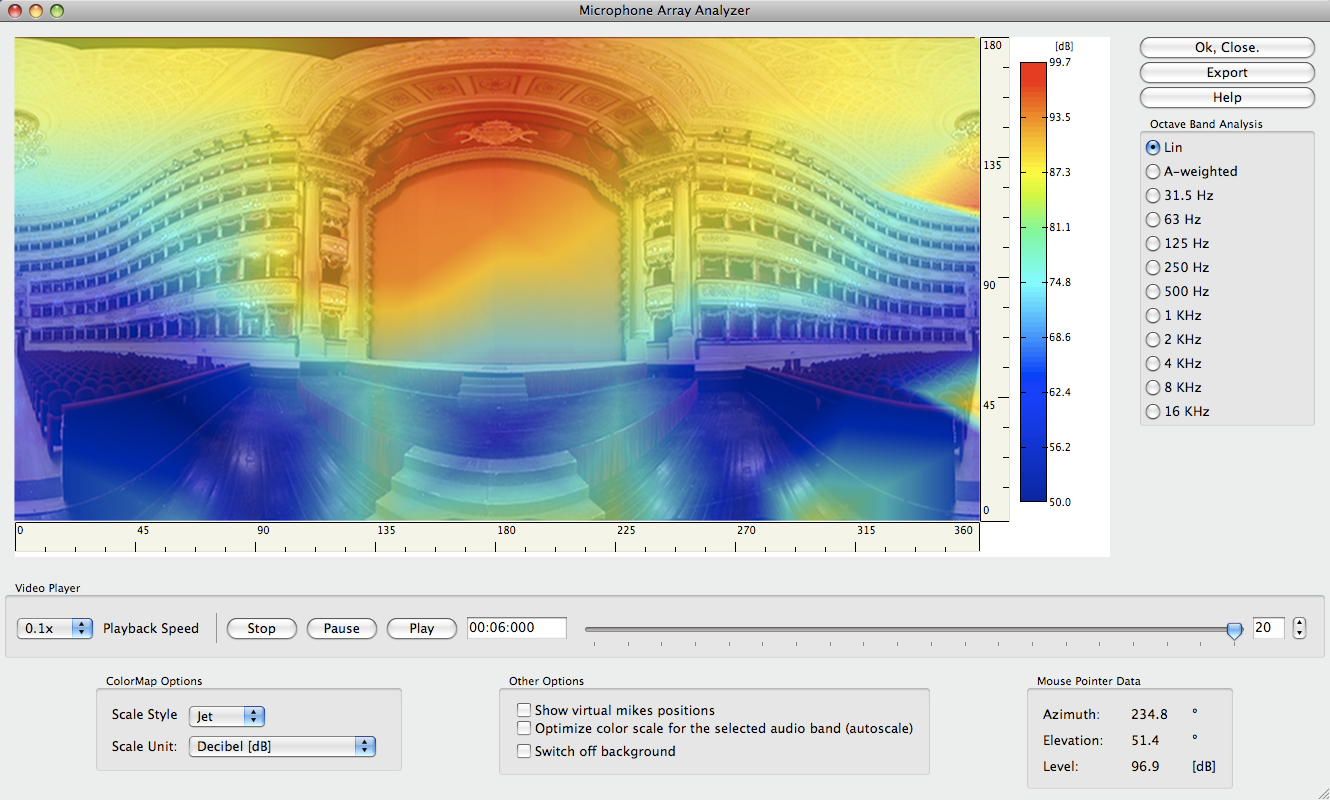
\includegraphics[width = 12cm]{img/maadlg.png}
  \caption{Finestra principale del modulo \emph{Microphone Array Analyzer}\\}
  \label{fig:maadlg}
\end{figure}
	Come possiamo notare in figura \ref{fig:maadlg}, la finestra principale del \emph{plug-in} mostra un video player contenente un video di output preliminare, ottenuto utilizzando un set di opzioni di default. 
	Si ha per� accesso anche a tutte queste opzioni direttamente dagli altri pannelli della finestra, potendo quindi modificare ciascuna di queste opzioni e di conseguenza il video di output.
	Si procede ora con la descrizione, una per una, di queste configurazioni ulteriormente disponibili:
		\begin{description}
 		 \item[Selettore di banda di frequenze] secondo cui filtrare i risultati e osservare quindi al meglio il comportamento delle onde sonore in una banda particolare. 
		 Si pu� quindi discriminare l'emissione di energia sonora in una particolare regione di spettro.
		 Questo tipo di analisi pu� essere molto utile quando si cerca di studiare un campo acustico dovendo discriminare diverse sorgenti sonore o particolari riflessioni di uno stesso impulso. Grazie al \emph{filtro passa-banda} � possibile eliminare dall'analisi del campo acustico tutto il materiale sonoro di minor interesse evidenziando quindi l'oggetto di attenzione in fase di test.
		 \item[Selettore di scala di colore] nella modalit� di un semplice men� a tendina che fornisce una gamma di tre possibilit� cromatiche, \emph{hot} o \emph{cold}, intuitivamente colori caldi o freddi, e \emph{jet} che invece passa dai freddi ai caldi mano a mano che aumenta il valore SPL che si vuole rappresentare.
		 Grazie a questa opzione � possibile variare la gradazione di colore usata per rappresentare i valori numerici sulla mappa, in modo da massimizzare il contrasto con il video sullo sfondo e rendere il grafico di pi� comoda interpretazione. 
		 Naturalmente, � possibile cambiare opzione anche durante la riproduzione video, come nel caso del cambio di \emph{filtro passa-banda} in modo da analizzare con due scale (o filtri) diversi due parti diverse del video.
		  \item[Selettore di unit� di misura] con cui rappresentare i livelli sonori. 
		  La scelta pu� ricadere in una delle quattro possibilit� offerte dal men� a tendina: decibel ($dB$), pascal ($Pa$), radice quadrata e cubica della pressione ($\sqrt{Pa}$ e $\sqrt[3]{Pa}$)
		  \item[Mostra/nascondi i microfoni virtuali] consente, selezionando l'apposita \emph{checkbox}, di visualizzare sulla colormap le posizioni dei microfoni virtuali contrassegnati da una piccola croce bianca.
		  \item[abilita/disabilita autoscale] permette di modificare i valori di massimo e minimo dei livelli SPL associati alla scala di colore rispettivamente considerando il massimo e minimo rispetto al materiale audio filtrato nella banda di frequenze attualmente selezionata, o semplicemente utilizzando i valori pre-filtraggio nel caso in cui la funzione di autoscale non sia selezionata.
		  Questo permette di apprezzare maggiormente i piccoli cambiamenti di livello di pressione misurati in punti vicini tra loro, al fine di notare maggiormente la direzione di provenienza di una sorgente piuttosto che di una riflessione particolare all'interno di un campo acustico complesso. Sar� sufficiente selezionare la banda di frequenze in cui risiede il suono che si vuole evidenziare per ottenere il risultato voluto.\footnote{\; Si noti che attraverso la medesima operazione � anche possibile effettuare l'analisi opposta e cio� risalire alla banda frequenziale di maggior rilievo in $dB$ per quanto riguarda il rumore di una sorgente di cui si conosce la direzione, magari nel caso in cui ci si trovi all'interno di un campo acustico complesso in cui � impossibile isolare la sola sorgente interessata.}
		  \item[disabilita/abilita lo sfondo] in modo da poter vedere correttamente i colori della mappa acustica senza \emph{l'interferenza} del video di background visibile in trasparenza. 
		  Per esempio potrebbe essere utile in casi complessi, poter visionare solo alcuni frame, \emph{spegnendo} il video di background, per poterlo poi riaccendere in seguito.
\end{description}
	Oltre a queste opzioni con cui personalizzare i risultati ottenuti, � presente nell'interfaccia grafica anche un ultimo pannello non interattivo che fornisce l'informazione riguardante il livello sonoro, nell'unit� di misura scelta, relativo alla posizione del mouse sulla mappa e quindi a una coordinata sferica nel gi� citato\footnote{ \;Secondo la norma ISO2631, come descritto al capitolo \ref{sec:eigensystem} e in figura \ref{fig:normaISO2631}} sistema di riferimento antropometrico centrato sull'array microfonico.
	
	Al termine delle operazioni, � possibile esportare i risultati tramite l'apposito bottone \emph{Esporta}.\\


		
	


%%%%%%%%%%%%%%%%%%%%%%%%%%%%%%%%%%%%%%%%%%%%%%%%%%%%%%%%%%%%%%%%%%%%%%%%%%%%%%%%%%%%%%%%%%%%%%%%%%%%%%%%%%%%%%%%%%%%%%%%%%%%%%%

%\begin{table}[htbp]
%   \centering
%   \begin{tabular}{l r r r r r r r}
%      $f_\textrm{cb}$ &   125 &   250 &   500 &  1000 &  2000 &  4000 &  8000 \\
%      \hline
%      \emph{SdF}      & -7.96 & -7.80 & -7.56 & -7.34 & -6.92 & -5.88 & -3.92 \\
%      \emph{SdP 1}    & -3.66 & -3.53 & -3.31 & -3.15 & -2.70 & -1.61 &  0.74 \\
%      \emph{SdP 2}    & -1.03 & -0.91 & -0.72 & -0.65 & -0.25 &  0.69 &  3.26 \\
%      \emph{SdP 3}    &  0.23 &  0.36 &  0.53 &  0.57 &  0.95 &  1.80 &  4.57 \\
%      \emph{SdP 4}    &  1.63 &  1.72 &  1.86 &  1.80 &  2.19 &  3.05 &  6.61 \\
%      \emph{SdP 5}   
%   \end{tabular}
%   \caption{$C_{80}$ per un ascoltatore situato a met\`a sala: confronto tra stato di fatto e gli stati di progetto elaborati}
%   \label{tab:c80mid}
%\end{table}

%\begin{table}[htbp]
%   \centering
%   \begin{tabular}{l r r r r r r r}
%      $f_\textrm{cb}$ &   125 &   250 &   500 &  1000 &  2000 &  4000 &  8000 \\
%      \hline
%      \emph{SdF}      & -7.58 & -7.45 & -7.22 & -7.04 & -6.65 & -5.68 & -3.73 \\
%      \emph{SdP 1}    & -5.85 & -5.72 & -5.49 & -5.33 & -4.87 & -3.81 & -1.28 \\
%      \emph{SdP 2}    & -2.29 & -2.17 & -1.95 & -1.85 & -1.42 & -0.42 &  2.33 \\
%      \emph{SdP 3}    & -1.29 & -1.12 & -0.88 & -0.81 & -0.33 &  0.75 &  4.04 \\
%      \emph{SdP 4}    &  0.79 &  0.90 &  1.08 &  1.03 &  1.49 &  2.49 &  6.50 \\
%      \emph{SdP 5}   
%   \end{tabular}
%   \caption{$C_{80}$ per un ascoltatore situato in fondo alla sala: confronto tra stato di fatto e gli stati di progetto elaborati}
%   \label{tab:c80far}
%\end{table}

      \chapter{Dettagli di Implementazione}
\label{sec:internalfunct}
	In questo capitolo si analizzeranno i dettagli del lavoro computazionale sotto il tracciamento della mappa. 
	La spiegazione del lavoro svolto seguir� i seguenti step:
 \begin{enumerate}
\item sintesi dei microfoni virtuali mediante convoluzione; 
\item scalatura delle ampiezze dei segnali risultanti in funzione del fondo 
scala specificato nella finestra di configurazione; 
\item mirroring dei microfoni virtuali, per garantire la continuit� ai bordi 
della mappa; 
\item copertura dell'intera area della mappa con superfici di forma 
triangolare (meshing); 
\item interpolazione dei dati ed il filtraggio in bande d'ottava; 
\item applicazione della scala colorata in relazione alla presenza o meno della 
funzione di auto-scaling. 
\end{enumerate}

Nei capitoli precedenti si � gi� analizzato lo step della sintesi dei microfoni virtuali mediante convoluzione (punto 1). Si proceder� di seguito con la spiegazione in dettaglio degli altri cinque passaggi.


	\section{Elaborazione numerica del suono}
	[lezione 12 ppt]\\
	
	[...]\\
	
	
	\section{Acquisizione del video}
	
	[...]\\
	
	
	\section{Livello di fondo scala}
	Il livello di fondo scala ($FS$) specificato dall'utente tramite la finestra di configurazione del plug-in, � inteso come livello massimo considerato dei segnali ottenuti dalla sintesi per convoluzione dei microfoni virtuali. 
	Per imporre il FS desiderato non � sufficiente una semplice amplificazione o attenuazione dei segnali di uscita, in quanto l'utente potrebbe aver selezionato uno spezzone casuale del segnale registrato, che quindi potrebbe non comprendere la regione di audio che causa il raggiungimento del livello di FS da parte dei segnali risultanti dalla convoluzione. 
	Per tenere conto di tale possibilit�, si utilizza un algoritmo che svolge le seguenti funzioni: 
	\begin{enumerate}
\item determina su quale canale $n$ del progetto Audacity\textregistered si ha il picco massimo 
di ampiezza tra tutti i canali registrati e ne memorizza il valore $ABS_{MAX-dB}$; 
\item determina il picco massimo di ampiezza dello stesso canale $n$, considerando solo il segnale entro la selezione, e ne memorizza il valore $REL_{MAX-dB}$;
\item determina il nuovo livello di FS corretto sfruttando la relazione:
		\begin{equation}
			FS_{FIX_dB}=FS_{USER_dB}-ABS_{MAX-dB}-REL_{MAX-dB}
		\end{equation}
\end{enumerate}
	In tal modo, il livello di $FS$ specificato dall'utente sar� riscalato in relazione al 
rapporto tra l'ampiezza massima assoluta del segnale, cio� quella determinata 
lungo la sua intera durata, e l'ampiezza massima relativa allo spezzone selezionato. 
	Grazie all'introduzione di questo algoritmo il \emph{plug-in} non deve calcolare l'intera convoluzione per poi, dopo aver applicato la correzione del FS, doverne scartare la maggior parte, ma viene svolta l�analisi solo sullo spezzone desiderato (??).
	
	\section{\emph{Mirroring} dei microfoni virtuali}
	\label{sec:mirroring}
	La registrazione effettuata con un array sferico non produce una mappa dei livelli sonori come proiezione cilindrica di una mappa sferica, come ad esempio una mappa ottenibile con un procedimento simile a quello usato per la rappresentazione della superficie terrestre sul planisfero. 
Muovendo dall'esempio del planisfero, � noto che, essendo la terra sferica, muovendosi lungo i bordi del planisfero si avr� una certa continuit� della mappa, ovvero uscendo da nord si rientrer� da sud, uscendo da est si rientrer� da ovest etc. 
Nel caso particolare di tracciamento della mappa sonora,si � proceduto prolungando la mappa stessa oltre i propri bordi. Per fare ci� si � effettuata una estensione della mappa \emph{specchiando} i punti relativi ai microfoni virtuali sintetizzati seguendo lo schema proposto da Binelli, Venturi, Amendola e Farina nel documento~\cite{spheric-soundfield} e riportato in Figura~\ref{fig:spheric}. 

%%%%%%%%%%%%%%%%%%%%%%%%%%%%%%%% FIGURA MIRRORING %%%%%%%%%%%%%%%%%%%%%%%%%%%%
\begin{figure}
  \centering
  \includegraphics[width = 11cm]{img/spheric.pdf}
  \caption{Rappresentazione schematica del processo di \emph{mirroring}, necessario a garantire la 
continuit� ai bordi della mappa.}
  \label{fig:spheric}
\end{figure}

	Dalla figura si osserva che i quattro quadranti in cui pu� essere scomposta la fotografia sferica, A, B, C e D, debbano essere \emph{copiati e specchiati}  verticalmente e/o orizzontalmente attorno alla fotografia, per imporre la condizione di continuit�; pi� precisamente si � proceduto copiando le posizioni e i livelli registrati dai microfoni virtuali in modo da riuscire a coprire con delle \emph{mesh} triangolari anche i bordi della mappa, cos� come meglio spiegato nel prossimo paragrafo.
	
	
	\section{\emph{Meshing} della superficie mediante l'operaizone di triangolazione di \emph{Delaunay}}
	\label{sec:delaunay}
	%%%%%%%%%%%%%%%%%%%%%%%%%%%%%%%% FIGURA CAPSULE %%%%%%%%%%%%%%%%%%%%%%%%%%%%
\begin{figure}
  \centering
  \includegraphics[width = 13cm]{img/capsules.pdf}
  \caption{Direzioni di puntamento delle capsule dell'Eigenmike sovrapposte ad una foto panoramica del Teatro alla Scala di Milano, svolta secondo lo schema di proiezione visto nella sezione~\ref{sec:mirroring}.}
  \label{fig:capsules}
\end{figure}
	Per eseguire l'interpolazione di una serie di livelli noti di una funzione in due variabili, l'ascissa e l'ordinata, occorre suddividere l'intero piano in aree pi� piccole di forma poligonale, aventi come vertici tre o pi� coppie di coordinate in cui i livelli siano noti; 
	occorre poi ipotizzare, per ciascuna di queste aree, che i livelli ai vertici facciano tutti parte di un'unica funzione notevole, ed infine calcolare i valori che tale funzione assume in tutti i punti compresi quelli di ognuna delle sottoaree in cui si � suddivisa la superficie. 
	Questo primo passaggio � detto \emph{meshing} della superficie, mentre le sottoaree che vanno a ricoprire l'intera superficie prendono il nome di \emph{mesh}. 
	
	Il primo passo da fare � stabilire il metodo da seguire per determinare la griglia, ovvero la forma geometrica delle \emph{mesh} in cui l'intero piano xy andr� suddiviso. 
La prima ipotesi potrebbe essere la suddivisione in aree di forma quadrata (come i meridiani e i paralleli del planisfero): questa ipotesi � valida se i microfoni virtuali, che costituiscono la griglia dei punti in cui i livelli sonori sono noti, sono disposti su una griglia uniforme. 

	Come si pu� notare dalla Figura~\ref{fig:capsules}, le posizioni delle capsule dell'Eigenmike\textregistered purtroppo non lo sono, e se anche cos� fosse, lo sviluppo del plug-in sotto l'ipotesi di griglia uniforme avrebbe portato alla realizzazione di un software utilizzabile per un numero limitato di disposizioni dei microfoni virtuali. 
	
	La seconda ipotesi � quella di suddividere l'intero piano xy in superfici di forma triangolare; 
	in questo modo, anche nel caso in cui le posizioni dei microfoni fossero disposte nella maniera pi� casuale possibile, si potr� sempre determinare un insieme continuo di triangoli che copra l'intera superficie. 
	Infatti Nel 1925 � stato dimostrato che ogni super�cie pu� essere triangolata ma questo pu� richiedere un numero in�nito di triangoli.
	Per effettuare questa operazione si � scelto quindi di utilizzare una triangolazione particolare detta di \emph{Delaunay} che � definita come segue:
	
	\emph{Una triangolazione di un insieme �nito di punti $P \subset R^2$ viene detta di Delaunay se il cerchio circoscritto ad ogni triangolo � vuoto, ovvero nessun punto di $P$ vi giace all�interno}. 
	
		%%%%%%%%%%%%%%%%%%%%%%%%%%%%%%%% FIGURA CAPSULE %%%%%%%%%%%%%%%%%%%%%%%%%%%%
\begin{figure}
  \centering
  \includegraphics[width = 8cm]{img/delaunay.png}
  \caption{Descrizione della propriet� dei triangoli formati con l'algoritmo di \emph{Delaunay}.}
  \label{fig:delaunay}
\end{figure}
	
	Sono diversi gli algoritmi che consentono di determinare, dato un insieme di punti sparsi su un piano, la triangolazione di Delaunay. 
	I principali, con complessit� differente in funzione del numero di punti da triangolare, sono: 
\begin{itemize}
\item  l'algoritmo incrementale; 

\item  l'algoritmo dividi et impera; 

\item  l'algoritmo Convex Hull. 

\end{itemize}
	
	Per il presente lavoro di tesi si � deciso di utilizzare una libreria esterna, denominata Triangle++, per implementare l'algoritmo di \emph{Delaunay}, essendo l�implementazione particolarmente impegnativa. 
Triangle++ � il nome del wrapper $C++$ della libreria $C$ \emph{Triangle}\footnote{Si veda \cite{triangle}}; esso fornisce la definizione di una classe molto semplice da utilizzare, la quale, dato un insieme di punti di cui si vuole conoscere la triangolazione, svolge autonomamente il calcolo delle mesh facendo uso di tutti e tre gli algoritmi sopraccitati. 	
	
	
	
	\section{Interpolazione dei valori acquisiti e filtraggio in bande d'ottava}
	
	Quando si sia calcolata una ipotetica partizione del piano xy in \emph{mesh} di forma triangolare, all'interno di ciascuna delle quali ci interessi conoscere i valori assunti dalla funzione incognita dei livelli sonori, occorre scegliere, tra le tante possibili, una e una sola funzione da utilizzare come stima approssimativa di quella incognita, imponendo che soddisfi i livelli noti presenti ai tre vertici della mesh. 
La soluzione pi� semplice � quella di scegliere come funzione approssimante l'equazione di un piano passante per tre punti generici.  
Il metodo di interpolazione che ne deriva va sotto il nome di \emph{interpolazione bilineare}. 

Sapendo che l'equazione generica di un piano pu� essere scritta nella forma: 
	
	\begin{equation}
	\label{eq:plane}
		z=A\cdot x + B\cdot y + C
	\end{equation}

	e chiamando ($x_{1i}$, $y_{1i}$, $z_{1i}$), ($x_{2i}$, $y_{2i}$, $z_{2i}$) e ($x_{3i}$, $y_{3i}$, $z_{3i}$) le coordinate degli unici tre punti noti della funzione incognita dei livelli sonori, dove i valori $z_{1i}$, $z_{2i}$ e $z_{3i}$ corrispondono proprio ai livelli misurati in corrispondenza dei tre vertici della i-esima mesh, l'imposizione del passaggio del piano per i tre punti corrisponde all'equazione matriciale: 
		\begin{equation}
		\label{eq:planefor3points}
		\left(\begin{array}{c c c }
		x_{1i} & y_{1i} & 1 \\
		x_{2i} & y_{2i} & 1 \\
		 x_{3i} & y_{3i} & 1 \\
		 \end{array}\right)
		 \cdot
		 \left(\begin{array}{c}A \\B \\C\end{array}\right)	
		 =
		 \left(\begin{array}{c}z_{1i} \\z_{2i} \\C\end{array}\right)
 	\end{equation}
	
%	che, attraverso semplici manipolazioni, pu� essere riscritta come:
%
%	\begin{equation}
%	\left(\begin{array}{c}A \\B \\C\end{array}\right)
%	=
%	\frac{1}{\det (M)}
%	\cdot
%	\left(\begin{array}{c}
%		z_{1i}\cdot (y_{2i} - y_{3i}) + z_{2i}\cdot (y_{3i} - y_{1i}) + z_{3i}\cdot (y_{1i} - y_{2i})  \\
%		z_{1i}\cdot (x_{3i} - x_{2i}) + z_{2i}\cdot (x_{1i} - x_{3i}) + z_{3i}\cdot (x_{2i} - x_{1i})  \\
%		z_{1i}\cdot (x_{2i}\cdot y_{3i} - x_{3i}\cdot y_{2i} ) + z_{2i}\cdot (x_{2i}\cdot y_{1i} - x_{1i}\cdot y_{3i} ) + z_{3i}\cdot (x_{1i}\cdot y_{2i} - x_{2i}\cdot y_{1i} ) 
%	\end{array}\right)	
%	\end{equation}

	L'equazione \ref{eq:planefor3points} rappresenta esattamente l'approccio utilizzato dalla classe \emph{TriangularMesh}, definita all'interno del codice del \emph{plug-in} progettato, per il calcolo dei coefficienti $A$, $B$, $C$ e $\det (M)$ che servono per l'interpolazione. 
	Quando si desiderer� conoscere il livello sonoro in una certa posizione di coordinate (in pixel) che cadono entro una certa \emph{mesh}, si dovr� chiamare la funzione membro dell'oggetto che rappresenta la \emph{mesh} di interesse e che, implementando la \ref{eq:planefor3points}, ci restituir� il valore interpolato.
	 
	Questa ipotesi sarebbe corretta nel caso in cui ad ogni vertice di ciascuna mesh fosse possibile associare un unico livello sonoro, ma ci� non pu� avvenire. 
	Come si � visto nel precedente capitolo 

(verificare)

	, infatti, il \emph{plug-in} consente di effettuare una analisi in bande d'ottava\footnote{si veda la sezione \ref{sec:band}} dei livelli sonori ovvero si avranno non una sola mappa dei livelli, bens� tante mappe quante sono le possibili bande d'ottava selezionabili. 
	Per risolvere occorre usare come terza "coordinata" di ciascun vertice il numero del microfono virtuale posizionato nelle stesse coordinate del vertice (anzich� il livello sonoro) e memorizzare una matrice dei livelli sonori tale che, incrociando il numero del microfono virtuale con il numero identificativo della banda selezionata, fornisca il livello sonoro corretto per la determinazione dei coefficienti $A$, $B$, $C$ e $\det (M)$ necessari per la costruzione della mappa della particolare banda selezionata. 
	Il processo di filtraggio � stato affrontato in modo trasparente grazie all'utilizzo di una classe gi� progettata per la suite di plug-in \emph{Aurora} per Audacity\textregistered \footnote{si veda \cite{aurora}} la quale gi� disponeva di tutte le funzioni membro necessarie ad implementare i filtraggi in bande d'ottava, come definiti secondo norma IEC-1260.
	Infine, dopo l�operazione di filtraggio, � necessario creare un \emph{frame audio} cio� una mappa statica che rappresenti il contenuto del campo acustico nell'intervallo non infinitesimo di un frame\footnote{selezionato dall'utente come al paragrafo \ref{sec:framelength}} del video che si sta andando a costruire; occorre qui un calcolo del valore \emph{RMS}\footnote{si veda l'appendice (da scrivere e da controllare se � la prima citazione-noncredo-) \ref{sec:rms}} dei segnali filtrati. 





	\section{Mappatura con scale cromatiche e \emph{auto-scaling}}
	
	La scala di colore che si utilizza � una funzione in una incognita a tre variabili dipendenti: l'incognita � il livello sonoro in un dato punto ed i tre valori di uscita della funzione coincidono con i tre canali $R$ ($red$), $G$ ($green$) e $B$ ($blue$) di una interfaccia video. 
	A seconda della scala di colore disederata, sar� utilizzata una \emph{routine} diversa per determinare il valore $RGB$ del pixel interessato, il quale sar� successivamente inserito in una \emph{mappa RGB} (una bitmap, appunto). 
	Per assegnare ai valori di $SPL$ un valore $RGB$ � necessario stabilire gli estremi SPL da rappresentare per poi successivamente effettuare tutta la scalatura tra i livelli in modo proporzionale. Infatti le relazioni tra i valori $R$, $G$ e $B$ e il livello che si vuole mappare sono parametrizzate in funzione dei valori di minimo e massimo rappresentabili. 
	Non si tratta di un operazione banalissima in quanto per definire univocamente questi valori � necessario analizzare tutto il video alla ricerca degli estremi.
	Questo comporta la perdita della possibilit� di lavorare in tempo reale con una registrazione (a meno di accontentarsi di approssimazioni\footnote{si potrebbe per esempio... }), sar� invece necessario analizzare un audio pre-registrato.
	Dopo aver calcolato tutti i livelli corrispondenti ai microfoni virtuali, filtrati per ogni banda, ed effettuata questa operazione per ogni singolo frame\footnote{ cio� in seguito al precalcolo descritto in questo capitolo}, il programma � in grado di ottenere e salvare in una struttura dati i valori di $SPL$ massimi e minimi per ogni banda e per ogni frame.
	In questo modo sar� possibile individuare gli estremi cercati.
	
	Con la funzione di \emph{auto-scaling} si modificano i valori minimi e massimi entro i quali verr� adattata la scala colorata in base alla banda frequenziale selezionata dall'utente.
	
	Nel caso in cui sia stata abilitata la funzione \emph{auto-scale}\footnote{con il \emph{checkbox} descritto nella sezione \ref{sec:options}}, saranno modificati i valori $RMS$ di minimo e massimo dei segnali prodotti dai microfoni virtuali limitando la ricerca in ogni frame ai soli valori riguardanti la banda selezionata; 
	se il livello minimo cos� calcolato dovesse essere inferiore a quello di soglia stabilito dall'utente\footnote{si veda il paragrafo \ref{sec:confdlg}}, si considerer� come valore minimo il valore di soglia. 
	
	Nel caso in cui invece la funzione \emph{auto-scale} sia disabilitata, il livello minimo verr� assunto pari a quello di soglia inserito dall'utente, mentre quello massimo verr� assunto pari al massimo assoluto tra i livelli $RMS$ prodotti dai vari microfoni virtuali in tutte le bande e fra tutti i singoli frame del video di output. 
	
	\section{Esportazione dei risultati}
	
	[...]\\
	
	

%%%%%%%%%%%%%%%%%%%%%%%%%%%%%%%%%%%%%%%%%%%%%%%%%%%%%%%%%%%%%%%%%%%%%%%%%%%%%%%%%%%%%%%%%%%%%%%%%%%%%%%%%%%%%%%%%%%%%%%%%%%%%%%

%\begin{table}[htbp]
%   \centering
%   \begin{tabular}{l r r r r r r r}
%      $f_\textrm{cb}$ &   125 &   250 &   500 &  1000 &  2000 &  4000 &  8000 \\
%      \hline
%      \emph{SdF}      & -7.96 & -7.80 & -7.56 & -7.34 & -6.92 & -5.88 & -3.92 \\
%      \emph{SdP 1}    & -3.66 & -3.53 & -3.31 & -3.15 & -2.70 & -1.61 &  0.74 \\
%      \emph{SdP 2}    & -1.03 & -0.91 & -0.72 & -0.65 & -0.25 &  0.69 &  3.26 \\
%      \emph{SdP 3}    &  0.23 &  0.36 &  0.53 &  0.57 &  0.95 &  1.80 &  4.57 \\
%      \emph{SdP 4}    &  1.63 &  1.72 &  1.86 &  1.80 &  2.19 &  3.05 &  6.61 \\
%      \emph{SdP 5}   
%   \end{tabular}
%   \caption{$C_{80}$ per un ascoltatore situato a met\`a sala: confronto tra stato di fatto e gli stati di progetto elaborati}
%   \label{tab:c80mid}
%\end{table}

%\begin{table}[htbp]
%   \centering
%   \begin{tabular}{l r r r r r r r}
%      $f_\textrm{cb}$ &   125 &   250 &   500 &  1000 &  2000 &  4000 &  8000 \\
%      \hline
%      \emph{SdF}      & -7.58 & -7.45 & -7.22 & -7.04 & -6.65 & -5.68 & -3.73 \\
%      \emph{SdP 1}    & -5.85 & -5.72 & -5.49 & -5.33 & -4.87 & -3.81 & -1.28 \\
%      \emph{SdP 2}    & -2.29 & -2.17 & -1.95 & -1.85 & -1.42 & -0.42 &  2.33 \\
%      \emph{SdP 3}    & -1.29 & -1.12 & -0.88 & -0.81 & -0.33 &  0.75 &  4.04 \\
%      \emph{SdP 4}    &  0.79 &  0.90 &  1.08 &  1.03 &  1.49 &  2.49 &  6.50 \\
%      \emph{SdP 5}   
%   \end{tabular}
%   \caption{$C_{80}$ per un ascoltatore situato in fondo alla sala: confronto tra stato di fatto e gli stati di progetto elaborati}
%   \label{tab:c80far}
%\end{table}

      \chapter{Conclusioni}
\label{sec:endings}
	In questo progetto di tesi si � lavorato alla scrittura di un software che fosse in grado di elaborare registrazioni multicanale prefiltrate, provenienti da un array microfonico generico, congiuntamente a una registrazione video dello stesso evento, in modo da generare in output una mappa sonora dinamica che fornisse una indicazione qualitativa dell'evoluzione del campo acustico.
	Come scelta di progetto � stata mantenuta la linea di implementare il software in forma di plug-in \audacity , piattaforma che permette ai suoi \emph{plug-ins} o \emph{moduli} di accedere a moltissime propriet� e dati del workspace, cosa non altrettanto vera per tutti gli altri standard diffusi di plug-in come per esempio i \emph{VST} e gli \emph{Audiounits}.

	Il plug-in progettato in questa sede � funzionante ed altamente interattivo, con svariate tipologie di realizzazione della mappa grazie alla possibilit� di configurare lo stile della scala di colore, la percentuale di trasparenza della mappa sovrapposta al video di background, l'unit� di misura dei livelli mostrati, i valori di fondo scala, la lunghezza del frame video, la percentuale di overlap tra i singoli frame etc.). 
	
	Dal confronto degli output del modulo in oggetto con altri calcolate dallo script Matlab\textsuperscript{\texttrademark} \; descritto nel documento \cite{spheric-soundfield} si � inoltre riscontrata una certa coerenza tra i risultati ottenuti; ben sapendo che non � ancora stato scoperto un metodo realmente applicabile per tarare una misura effettuata con un array microfonico, si desume che i risultati ottenuti con l�uso del \emph{plug-in} siano corretti. 

	In futuro, se si riuscisse a scoprire questo metodo di taratura per array microfonici, sarebbe possibile utilizzare il plugin in modo molto efficace in campo rumoristico per effettuare misure di livelli sonori.

% Appendixes
\appendix
\renewcommand{\chaptermark}[1]{\markboth{{\appendixname}\ \thechapter.\hspace{1em}#1}{}}
      \chapter{Appendice}
\label{se:appendix}

In questa appendice finale si trovano tutte le definizioni teoriche indispensabili alla comprensione dell'elaborato qui presentato ma il cui studio � considerato prerequisito e quindi noto. Viene dunque riportato un breve riassunto delle nozioni fondamentali in modo da fornire un quadro generale ristretto ma comunque sufficiente per affrontare serenamente la lettura.

\section{Propagazione di onde sonore}
\label{sec:wavesprop}

Un'onda sonora\footnote{Vedi \cite{amea}, capitolo 3.}, come risaputo, \`e una 
perturbazione della pressione atmosferica 
avente la propriet\`a di propagarsi; affinch\'e questo possa avvenire occorrono
due elementi indispensabili: una causa ed un mezzo. Il primo potr\`a essere un
sistema meccanico oscillante con sufficiente 
frequenza\footnote{Un'onda di pressione
   perch\'e venga percepita dall'apparato uditivo umano deve avere frequenza compresa
   tra 20 Hz e 20000 Hz circa, a seconda dell'individuo.}, mentre il secondo \`e,
in generale, un fluido, di norma l'aria.\\
La descrizione fisica della propagazione delle onde suddette avviene tramite 3
leggi fondamentali che di seguito si riassumono:

\begin{description}
  \item[L'equazione di Eulero.]  Siano $p$ la pressione sonora, $\mathbf{u}$ il vettore velocit\`a
        istantanea di una particella di fluido e $\rho_0$ la densit\`a dell'aria in condizioni normali,
	allora si ha:

        \begin{equation}
	  \label{eq:eulerlaw}
	  \nabla p = - \rho_0 \frac{\partial \mathbf{u}}{\partial t}.
	\end{equation}

	La relazione~\ref{eq:eulerlaw} altro non \`e che l'equivalente fluidodinamico della seconda legge
        newtoniana della dinamica, da cui deriva, ed esprime in sostanza le condizioni di equilibrio
	dinamico delle forze agenti su un elemento di fluido.

 \item[L'equazione di continuit\`a.] Se si esprime con $\delta$ la variazione relativa di densit\`a, o 
      \emph{condensazione}\footnote{\`E data da

          \begin{displaymath}
	     \delta = \frac{\rho - \rho_0}{\rho}
          \end{displaymath}

	  dove $\rho$ \`e densit\`a dell'elemento di fluido considerato.}, del mezzo
      e con $\mathbf{s}$ il vettore spostamento, per un generico elemento di fluido vale la legge

      \begin{equation}
	\label{eq:continuity}
	\delta = - \nabla \cdot \mathbf{s},
      \end{equation}

      che sintetizza il principio secondo cui il flusso netto di massa, ossia la differenza tra quello
      entrante e quello uscente, deve essere uguagliato dalla variazione di massa di fluido
      contenuta dall'elemento.

 \item[L'equazione di stato termodinamico.] Ipotizzando ragionevolmente variazioni di stato talmente
      rapide da poter essere ritenute adiabatiche ed indicando con $p_0$ il valore della pressione sonora
      a riposo e con $\gamma$ il rapporto tra i calori specifici del gas, rispettivamente, a pressione e
      volume costante, il comportamento termodinamico del fluido in questione \`e dato da

      \begin{equation}
	\label{eq:statelaw}
	\frac{1}{p_0} \frac{\partial p}{\partial t} = \gamma \frac{\partial \delta}{\partial t}.
      \end{equation}

\end{description}

Dalle relazioni~\ref{eq:eulerlaw}, \ref{eq:continuity} e~\ref{eq:statelaw}, dopo qualche passaggio, si
ricava l'\emph{equazione di propagazione delle onde sonore}:

\begin{equation}
  \label{eq:wavelaw}
  \nabla^2 p = \frac{1}{c^2} \frac{\partial^2 p}{\partial t^2},
\end{equation}

in cui $c$ \`e la velocit\`a di propagazione dell'onda sonora nel gas, definita come

\begin{equation}
  \label{eq:soundspeed}
  c = \sqrt{\gamma \frac{p_0}{\rho_0}}.
\end{equation}


%%%%%%%%%%%%%%%%%%%%%%%%%%%%%%%%%%%%%%%%%%%%%%%%%%%%%%%%%%%%%%%%%%%%%%%%%%%%%%%%%%%%%%%%%%%%%%%%%%%%%%%

\section{Intensit\`a, densit\`a di energia e potenza}
\label{sec:power}

Di seguito si riportano le definizioni di alcune grandezze fondamentali\footnote{Per i dettagli si
    rimanda sempre a~\cite{amea}.}:

\begin{description}

  \item[Intensit\`a sonora.] \`E la quantit\`a di energia che fluisce, nell'unit\`a di tempo, attraverso una
       superficie di area unitaria perpendicolare alla direzione di propagazione dell'onda. L'\emph{intensit\`a
       istantanea} \`e data da

       \begin{equation}
	 \label{eq:istint}
         I = p_m u_m \cos^2 \left[ \omega \left( t - \frac{x}{c} \right) \right],
       \end{equation}

       dove $p_m$ e $u_m$ sono i valori di picco di pressione e velocit\`a relative alla direzione di
       propagazione considerata, mentre l'\emph{intensit\`a media} dalla relazione

       \begin{equation}
	 \label{eq:meanint}
         \overline{I} =\frac{p_\textrm{rms}}{\rho_0 c} \quad \left[ \frac{\textrm{W}}{\um^2} \right].
       \end{equation}


       La quasi totalit\`a delle sorgenti reali, per\`o, non irradia energia uniformemente in tutte le direzioni,
       tale caratteristica viene misurata da una grandezza denominata \emph{direttivit\`a} ed indicata con
       $Q$; si ha

       \begin{equation}
	 \label{eq:directivity}
          Q = \frac{I_{\theta, \phi}}{\overline{I}},
       \end{equation}

       dove $I_{\theta, \phi}$ \`e l'intensit\`a irradiata nella direzione specificata, in coordinate sferiche,
       dagli angoli $\theta$ e $\phi$.

  \item[Densit\`a di energia sonora.] \`E l'energia contenute in un'unit\`a di volume del mezzo ed \`e data
       da

       \begin{equation}
	 \label{eq:density}
         D = \frac{\overline{I}}{c^2} =\frac{p_\textrm{rms}}{\rho_0 c^2} 
	                               \quad \left[ \frac{\textrm{W} \cdot \textrm{s}}{\um^3} \right].
       \end{equation}

  \item[Potenza sonora.] Supponendo che tutta l'energia sonora fluente nel mezzo sia prodotta da una sola e
       ben identificabile sorgente, l'energia irradiata nell'unit\`a di tempo da quest'ultima rappresenta
       la sua potenza sonora $W$. Se $S$ \`e una superficie immaginaria inviluppante la sorgente ed $I_S$
       l'intensit\`a sonora rilevata su un area elementare $\ud S$ della superficie, risulta

       \begin{equation}
	 \label{eq:power}
          W = \int_S I_s \, \ud S.
       \end{equation}


\end{description}

%%%%%%%%%%%%%%%%%%%%%%%%%%%%%%%%%%%%%%%%%%%%%%%%%%%%%%%%%%%%%%%%%%%%%%%%%%%%%%%%%%%%%%%%%%%%%%%%%%%%%%%

\section{Livelli sonori}
\label{sec:levels}

Per via dell'enorme capacit\`a dinamica dell'orecchio umano difficilmente viene adottata la scala
lineare per rappresentare le grandezze acustiche: dovendo trattare con un campo di valori estremamente
esteso e disperso\footnote{La minima pressione percepibile da un individuo normo udente \`e di 20 $\mu$Pa,
   la soglia del dolore \`e, invece, attorno ai 60 Pa.} \`e universalmente preferita la scala dei decibel,
codificata nella norma ISO 1648. Premettendo che un valore espresso in decibel implica \emph{sempre} un
rapporto con un altro valore di riferimento, di seguito si riportano le principali grandezze impiegate:

\begin{description}
  \item[Livello di pressione sonora.]

       \begin{eqnarray}
	 \label{eq:pressurelevel}
          L_p & = & 10 \log \frac{p^2}{p_0^2} = \nonumber \\
              & = & 20 \log \frac{p}{p_0} \quad \textrm{[dB]},
       \end{eqnarray}

       dove $p_0 = 20 \, \mu$Pa. La~\ref{eq:pressurelevel} si pu\`o anche riscrivere nel seguente modo,
       dopo aver sostituito il valore di $p_0$:

       \begin{equation}
	 \label{eq:pressurelevel2}
	 L_p = 10 \log p^2 + 94 \quad \textrm{[dB]}.
       \end{equation}

  \item[Livello di potenza sonora.]

       \begin{equation}
	 \label{eq:powerlevel}
          L_W = 10 \log \frac{W}{W_0} \quad \textrm{[dB]},
       \end{equation}

       dove $W_0 = 1$ pW. Sostituendo quest'ultimo valore nella~\ref{eq:powerlevel} si ricava

      \begin{equation}
	 \label{eq:powerlevel2}
          L_W = 10 \log W + 120 \quad \textrm{[dB]}.
       \end{equation}

  \item[Livello di intensit\`a sonora.]
  
     \begin{equation}
	 \label{eq:intensitylevel}
          L_I = 10 \log \frac{I}{I_0} \quad \textrm{[dB]},
       \end{equation}

      dove $I_0 = 1$ pW/m$^2$.  \`E largamente in uso esprimere anche la direttivit\`a in decibel: in questo
      caso il parametro definito dall'equazione~\ref{eq:directivity} prende il nome di 
      \emph{Directivity Index} ed \`e cos\`i definito

      \begin{eqnarray}
	\label{eq:dirindex}
        \textit{DI} & = & 10 \log Q  = \nonumber \\
	            & = & L_{I_{\theta, \phi}} - L_{\overline{I}}.
       \end{eqnarray}

\end{description}

Se $\rho_0 c$ vale 400 rayl risulteranno uguali $\rho_0 c I_0$ e $p_0^2$, cio\`e sar\`a verificata la
relazione 

\begin{equation}
  \label{eq:lieqlp}
  L_I = L_p.
\end{equation}

Tale situazione si avrebbe a pressione atmosferica e temperatura di 39$^\circ$C; alla temperatura di
20$^\circ$C il valore dell'impedenza acustica sale a 415 rayl, tuttavia l'errore commesso applicando
ugualmente la~\ref{eq:lieqlp} \`e comunemente ritenuto trascurabile.\\
Se l'intensit\`a sonora $I$ \`e uniforme su una superficie $S$ che circoscrive una sorgente di potenza
$W$ si pu\`o scrivere:

\begin{equation}
  \label{eq:lweqlieqls}
  10 \log \frac{W}{W_0} = 10 \log \frac{I}{I_0} + 10 \log \frac{S}{S_0} \quad \textrm{[dB]};
\end{equation}

se, poi, $S_0 = S = 1 \, \um^2$, risulta esattamente 

\begin{equation}
  \label{eq:lweqli}
  L_W = L_I.
\end{equation}

%%%%%%%%%%%%%%%%%%%%%%%%%%%%%%%%%%%%%%%%%%%%%%%%%%%%%%%%%%%%%%%%%%%%%%%%%%%%%%%%%%%%%%%%%%%%%%%%%%%%%%%

\section{Curve di ponderazione}
\label{sec:pondcurves}

La sensibilit\`a dell'orecchio umano non \`e costante in tutta la banda udibile, ma presenta un massimo
nella regione attorno a 4 kHz ed ha i valori minimi in corrispondenza degli estremi, come evidenziato
dalle curve isofoniche elaborate da Fletcher e Munson.\footnote{Si veda~\cite{mdaa} al capitolo 2.}
Questo ha portato all'ideazione delle unit\`a di misura \emph{percettive} (la scala dei \emph{phon})
ed ha suggerito l'adozione negli strumenti di misura di un filtraggio dei livelli rilevati in modo
da renderli coerenti alla reale sensibilit\`a umana. Il suddetto filtraggio \`e codificato nelle
cosiddette \emph{curve di ponderazione}, le quali non fanno altro che indicare l'alterazione della
risposta in frequenza dello strumento, ossia il fattore con cui debbono essere pesate le frequenze
della banda audio. In figura~\ref{fig:ponderaz} sono riportate le curve di ponderazione A, B e C
che sono, sostanzialmente, le curve isofoniche a 40, 70 e 100 phon rispettivamente.


%%%%%%%%%%%%%%%%%%%%%%%%%%%%%%%%%%%%%%%%%%%%%%%%%%%%%%%%%%%%%%%%%%%%%%%%%%%%%%%%%%%%%%%%%%%%%%%%%%%%%%%

\section{Trasformata di Fourier}
\label{sec:fourier}

L'argomento \`e enorme, in questa sede se ne vuole solo riportare la definizione operativa.
Se $x(t)$ \`e una funzione 

\begin{itemize}   
   \item limitata
   \item tale da presentare un numero finito di discontinuit\`a 
   \item assolutamente integrabile  
\end{itemize}

allora la sua trasformata secondo Fourier \`e data dalla relazione 

\begin{equation}
 \label{eq:fourier}
  X(f) = \int_{-\infty}^{\infty} x(t) \, e^{-j2\pi ft} \, \ud t.
\end{equation}

La trasformata inversa del segnale $X(f)$, invece si pu\`o calcolare mediante l'equazione

\begin{equation}
  \label{eq:invfourier}
  x(t) = \int_{-\infty}^{\infty} X(f) \, e^{j2\pi ft} \, \ud f.
\end{equation}

In generale affinch\`e esista la trasformata di Fourier del segnale $x(t)$, per il teorema di Plancherel \`e sufficiente 
che quest'ultimo abbia energia finita, caratteristica, questa, di tutti i segnali fisici.\\




% Bibliography
\bibliographystyle{siamcst}
\bibliography{public}


%Thanksgiving
    \newpage
\vspace*{10pc}
\pagestyle{empty}
\linespread{1}
\em

Se proprio devo ringraziare...

\par\vfill\par

\newpage

\vspace*{9cm}
\thispagestyle{empty}
\centering
\em
Typesetted on 2013 September 27 with \LaTeXe

\end{document}